%%=============================================================================
%% Methodologie
%%=============================================================================

\chapter{De werking van Kotlin/Native}
JetBrains heeft met Kotlin/Native de interesse van elke cross-platform ontwikkelaar getrokken. Niemand had verwacht dat Kotlin uitgebreid ging worden met een cross-platform framework. Zo zal JetBrains met Kotlin/Native een nieuwe markt betreden, het maken van native applicaties in combinatie met het delen van domeinlogica tussen de verschillende ondersteunde platformen.
\label{ch:kotlinnative}

\section{Wat is Kotlin/Native?}
Kotlin/Native is een technologie die zorgt voor de compilatie van Kotlin naar native binaire bestanden die zonder VM draaien. Kotlin/Native maakt gebruikt van een LLVM gebasseerde backend voor de Kotlin-compiler en een native implementatie van de Kotlin bibliotheek. Origineel werd Kotlin/Native uitgevonden om compilatie van Kotlin mogelijk te maken op platformen die geen virtuele machines, zoals de JVM, ondersteunen. Een voorbeeld hiervan is iOS dat geen ondersteuning biedt voor de JVM.

\iffalse
%TODO: Vragen
Kotlin Native ondersteunt volledig de interoperabiliteit met native code. Wat betreft het gebruik van Kotlin libraries, deze zijn volledig ter beschikking van de ontwikkelaar. Indien een bepaalde bibliotheek niet ondersteund wordt, bestaat er een tool om een tussenliggende bibliotheek te genereren van een C-header bestand, waardoor deze bibliotheek toch gebruikt kan worden.  Op macOS en iOS wordt samenwerking met Objective/C-code ook ondersteund.
\fi

Kotlin Native is momenteel heel jong en zit nog in volledige ontwikkeling. De eerste versie van Kotlin/Native werd vrijgegeven op 31 maart 2017. Er zijn reeds enkele versies aanwezig op de GitHub van JetBrains waar ontwikkelaars met aan de slag kunnen. De ondersteuning voor de IDE's is beschikbaar als een plugin voor CLion.

\section{Het delen van code in Kotlin/Native}
\label{sec:sharingcode}
Het doel van Kotlin/Native is om een framework aan te bieden dat gebruikt kan worden voor cross-platform ontwikkeling. De focus ligt niet op het maken van user interfaces, met alle functionaliteiten inbegrepen, via één codebase, maar wel op het delen van de domeinlogica. JetBrains wil dus via Kotlin/Native de mogelijkheid aanreiken om alle domeinlogica in een applicatie te hergebruiken op verschillende platformen en per platform de user interface op te bouwen.

Voordelen:
\begin{itemize}
	\item Hergebruik van de domeinlogica.
	\item Mogelijkheid om per platform, in de user interface, andere accenten naar voor te brengen.
\end{itemize}

Nadelen:
\begin{itemize}
	\item Verplichting om meerdere user interfaces op te bouwen (indien men meerdere platformen wil ondersteunen).
	\item Grotere kosten en meer tijd nodig om beide applicaties te ontwikkelen (Android en iOS).
	\item Opzet van dit soort projecten is (momenteel) niet gemakkelijk voor de onervaren gebruiker.
\end{itemize}

Figuur \ref{fig:sharingcode} toont hoe Kotlin/Native domeinlogica deelt over de verschillende platformen heen. Er wordt gebruik gemaakt van een \textbf{common} module. In deze module bevindt zich de gemeenschappelijke code, die gedeeld wordt met alle platformen en dus voor elk platform hetzelfde zal zijn. Daarnaast is er per platform dat ondersteund moet worden een aparte platformmodule. Deze platformmodules maken gebruik van de common module en er kan in deze platformmodules platformspecifieke code geschreven worden. De mogelijkheid is dus aanwezig om voor een bepaalde klasse, per platform een andere implementatie te voorzien. Zie sectie \ref{sec:expectandactual} voor een meer technische uitleg.

\begin{figure} [ht]
	\centering
	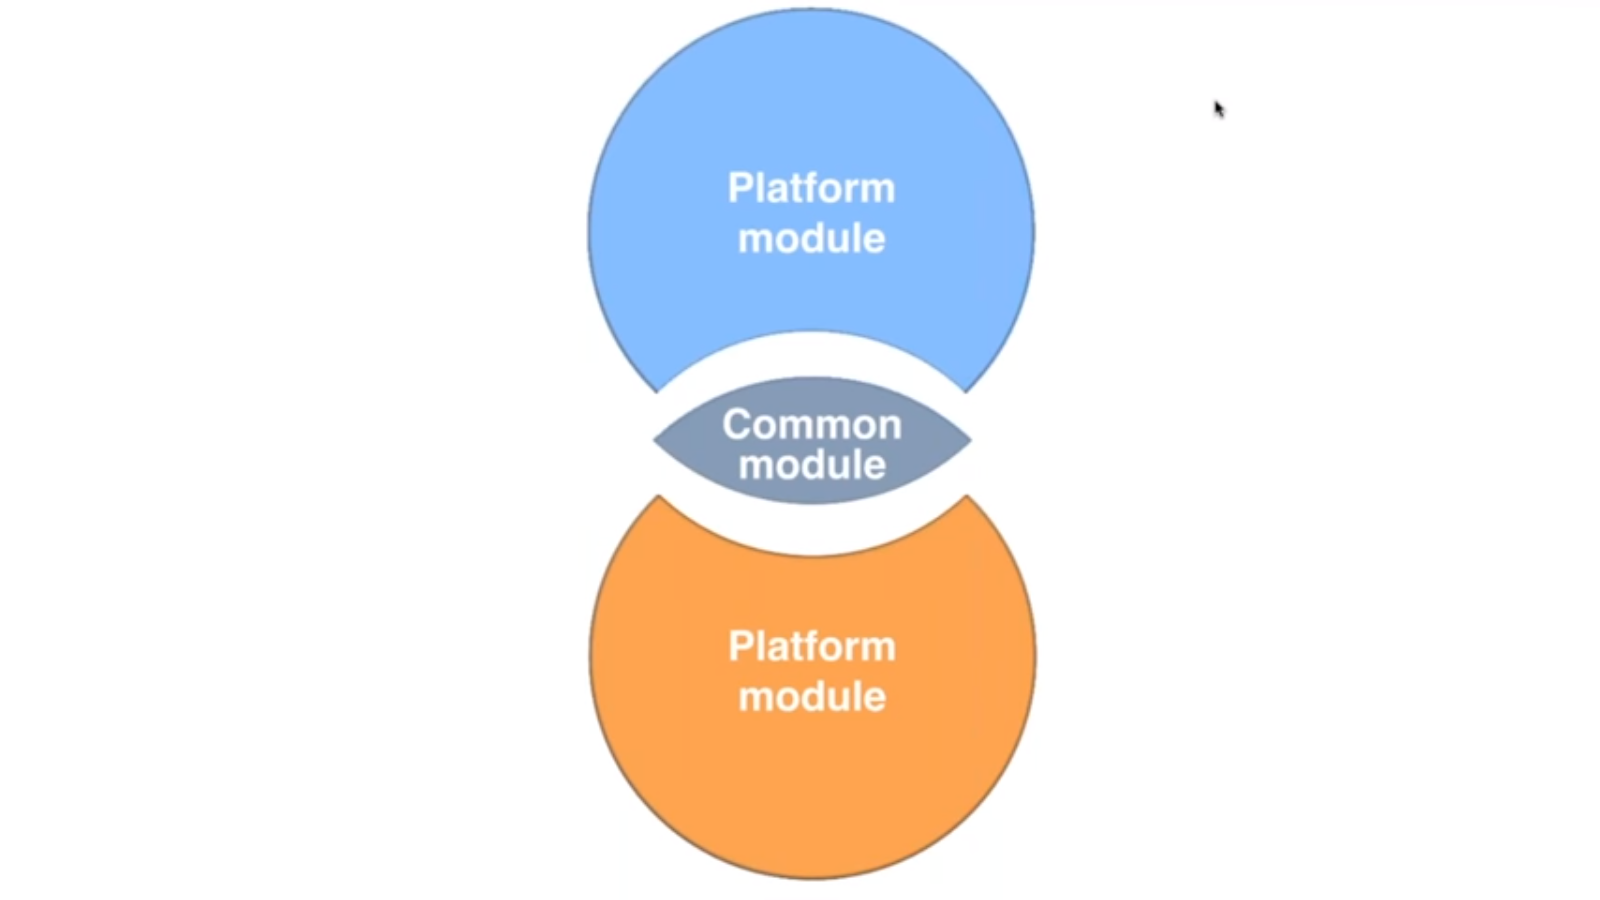
\includegraphics[width=0.95\textwidth]{img/sharingcode}
	\caption{Het delen van code in Kotlin Native (\cite{Developine})}
	\label{fig:sharingcode}
\end{figure}

\section{De structuur van een Kotlin/Native project}
\label{sec:knstructure}
Alvorens te beginnen met het ontwikkelen van een Kotlin/Native project is het belangrijk om na te gaan wat de structuur is waar een Kotlin/Native project moet aan voldoen. Er is namelijk geen IDE of plugin die een Kotlin/Native project volledig automatisch genereert, daarom is het essentieel dat er vanaf het begin een goede mappenstructuur wordt opgebouwd. Figuur \ref{fig:knstructuur} toont een goede structuur van een Kotlin/Native project. Deze mappenstructuur is verplicht om aan te houden, de namen van de mappen kunnen veranderd worden mits ook kleine verandering van de build scripts in \ref{ch:praktisch}.

\begin{figure} [ht]
	\centering
	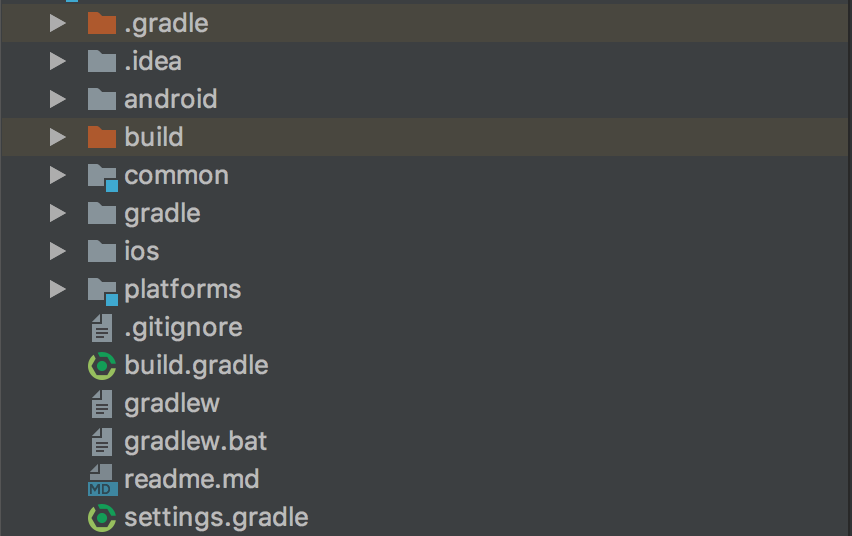
\includegraphics[width=0.95\textwidth]{img/kn-project-structure}
	\caption{Kotlin/Native structuur}
	\label{fig:knstructuur}
\end{figure}

Op deze figuur zijn dus een aantal mappen te vinden:
\begin{itemize}
	\item De \textbf{.gradle} map, automatisch gegenereerd, houdt alle instellingen en andere bestanden bij die gebruikt worden door Gradle om het project te bouwen. Dit wordt automatisch gegenereerd wanneer er een Gradle run wordt uitgevoerd.
	\item Voor dit voorbeeld werd IntelliJ gebruikt als IDE. IntelliJ zal de map, \textbf{.idea}, automatisch genereren om verschillende instellingen van het project bij te houden. Alle projectspecifieke instellingen zijn aanwezig in deze map.
	\item \textbf{android} bevat het volledige Android project.
	\item De \textbf{build} map bevat informatie over de laatste uitgevoerd build.
	\item De \textbf{common} map bevat gemeenschappelijke code dat over de verschillende platformen wordt gedeeld.
	\item De \textbf{gradle} map, automatisch gegenereerd, bevat een properties bestand. In dit bestand worden enkele belangrijke properties onthouden, zoals de locatie van de gradle installatie.
	\item \textbf{ios} bevat het volledige iOS project.
	\item De \textbf{platforms} map bevat voor ieder platform, dat men wenst te ondersteunen, een map. In dit voorbeeld zijn er dus twee mappen, een iOS en Android-map. De bedoeling is om hierin specifieke code te schrijven die varieert per platform. Zie sectie \ref{sec:sharingcode} voor meer informatie.
\end{itemize}

\section{Kotlin/Native code}
\subsection {Expect en actual klassen}
\label{sec:expectandactual}
Stel dat men wenst om een ABCMethods Kotlin klasse te hebben die de methodes callA(), callB() en callC() heeft, maar waarvan de implementatie verschillend is per platform.

In de common module wordt de ABCMethods klasse aangemaakt. Hierbij wordt het keyword \textit{expect} gebruikt. Het keyword zegt bijna zelf waarvoor het gebruikt moet worden: er wordt een ABCMethods klasse 'verwacht' voor ieder platform. Het expect keyword kan ook vergeleken worden met een standaard Java interface.

\begin{lstlisting}
expect class ABCMethods() {
	fun callA():String
	fun callB():String
	fun callC():String
}
\end{lstlisting}

Met het \textbf{actual} keyword geven we aan dat deze klasse een concrete implementatie is van ABCMethods. De compiler zal in eerste instantie zoeken naar de ABCMethods klasse in de common module. Hij zal daar merken dat ABCMethods een expect klasse is waardoor hij naar de platformspecifieke folder zal gaan en daar de actual klasse van ABCMethods zal gebruiken. Voor ieder platform wordt dus een concrete implementatie voorzien van de ABCMethods klasse.

Een mogelijke implementatie voor iOS:
\begin{lstlisting}
actual class ABCMethods actual constructor() {
	actual fun callA():String {
		return "Calling A from iOS"
	}
	
	actual fun callB():String {
		return "Calling B from iOS"
	}
	
	actual fun callC():String {
		return "Calling C from iOS"
	}
}
\end{lstlisting}

Een mogelijke implementatie voor Android:
\begin{lstlisting}
actual class ABCMethods actual constructor() {
	actual fun callA():String {
		return "Calling A from Android"
	}
	
	actual fun callB():String {
		return "Calling B from Android"
	}
	
	actual fun callC():String {
		return "Calling C from Android"
	}
}
\end{lstlisting}

Door gebruik te maken van Kotlin/Native is het niet nodig om zelf aan te geven welk bestand de compiler moet gebruiken voor welk platform. De compiler zal detecteren welk platform er gebruikt wordt en het juiste bestand gebruiken.

\subsection{Gemeenschappelijke klassen}
Naast de expect en actual klassen, die ervoor zorgen dat we platformspecifieke code kunnen schrijven en dus een onderscheid kunnen maken tussen de verschillende ondersteunde platformen, kunnen we ook klassen voorzien die voor alle platformen hetzelfde zijn. De implementatie van deze klasse is voor ieder platform hetzelfde.

\begin{lstlisting}
class Example {
	private var name: String
	
	constructor() {
		this.name = "Ilias.vw"
	}
	
	fun helloKotlin(): String {
		return "Hello Kotlin Native, from $name"
	}
}
\end{lstlisting}

\section {Het gebruiken van de Kotlin code}
\label{sec:use-ios-code}
Maar hoe kan de gemeenschappelijke en platformspecifieke code gebruikt worden? Simpel. Bij een Android-project kunnen we de Kotlin code gebruiken door simpelweg de bibliotheek te importeren. Dit is niks meer dan een import bovenaan in de Android activity. iOS gerelateerde code zal gedeeld worden via een iOS framework dat gegenereerd wordt door Kotlin/Native. Dit framework zal toegevoegd worden in de build phases van het Xcode project. Zie sectie \ref{sec:ios-stap6} voor meer informatie.

Kotlin/Native zal de code uit de common map en de code uit de platformspecifieke map bundelen tot één geheel. Zoals reeds gezegd zal dit bij iOS een framework zijn, bij Android echter een package die kan worden geïmporteerd. Dit gebeurt aan de hand van verschillende plugins, zie hoofdstuk \ref{ch:praktisch} voor meer informatie over deze build scripts.